Dzisiejsze interfejsy graficzne są projektowane zgodnie zasadami User Experience oraz User Interface. Są to zbiory wytycznych dla projektantów skoncentrowane na doświadczeniach użytkownika końcowego. User Experience to dziedzina zajmująca się badaniem potrzeb użytkownika, natomiast User Interface odpowiada za szatę graficzną produktu \cite{uxui}. ZodiaCal zostało stworzone zgodnie z powyższymi zasadami. Poniżej znajdują się Wireframes, czyli modele szkieletowe, zwane również jako architektura widoku aplikacji przedstawiające projekt graficzny poszczególnych ekranów wykonem w aplikacji internetowej Figma. Są to High-Fidelity Wireframes, co oznacza, że stanowią dopracowane rozwiązanie z szczegółowymi detalami \cite{uxui}.


\begin{figure}[h]
	\begin{minipage}{0.3\textwidth}
		\centering
		
\includegraphics[height=4cm, keepaspectratio]{images/logo/logo_text}
		\caption{Logo wraz z typografią}
		\label{fig:logo_text}
	\end{minipage}
	\hfill
	\begin{minipage}{0.3\textwidth}
		\centering
		
\includegraphics[height=4cm, keepaspectratio]{images/logo/logo}
		\caption{Logo bez typografii}
		\label{fig:logo}
	\end{minipage}
	\hfill
	\begin{minipage}{0.3\textwidth}
		\centering
		
\includegraphics[height=4cm, keepaspectratio]{images/logo/favicon}
		\caption{Ikona aplikacji favicon}
		\label{fig:favicon}
	\end{minipage}
\end{figure}

Rysunek \ref{fig:logo_text} przedstawia logo aplikacji ZodiaCal. Zostało one zaprojektowane z wykorzystaniem narzędzia Figma, który umożliwia tworzenie obrazów wektorowych, to znaczy obrazów opisanych za pomocą kształtów, linii i krawędzi w odróżnieniu do grafiki rastrowej opartej na pikselach. Dzięki wykorzystaniu wektorów grafiki nie tracą swojej ostrości
podczas powiększani, czy zmieniania obiektu. Stworzone logo miała nawiązywać do astrologicznych motywów tak, aby przywodziło na myśl horoskopy oraz wróżbiarstwo. Font wykorzystany do nazwy aplikacji został staranie wybrany, aby oddać charakter aplikacji. Jest to
font szeryfowy posiadający małe dekoracyjne elementy. Wykorzystanie takie rodzaju typografii ma na celu wywołanie wrażenia, że aplikacja prezentuje się w sposób klasyczny i elegancki.


\begin{figure}[t]
	\begin{minipage}{0.4\textwidth}
		\centering
		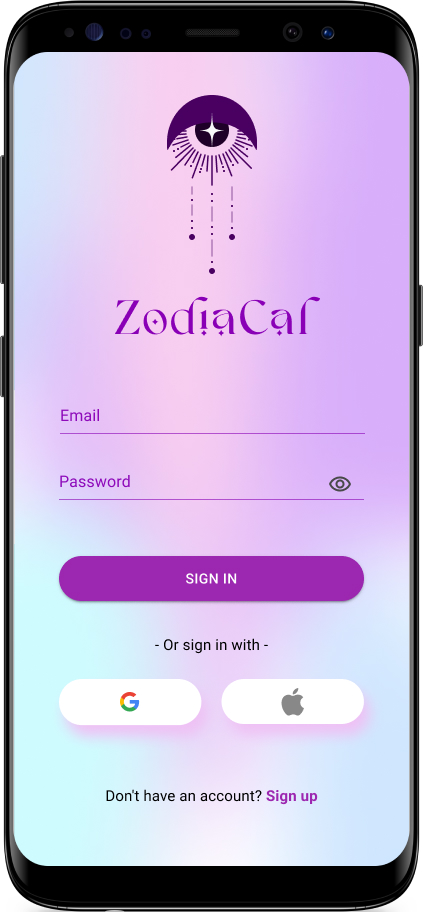
\includegraphics[height=10cm, keepaspectratio]{images/interfejs_figma/Sign_in}
		\caption{Ekran logowania}
		\label{fig:Sign-in}
	\end{minipage}
	\hfill
	\begin{minipage}{0.4\textwidth}
		\centering
		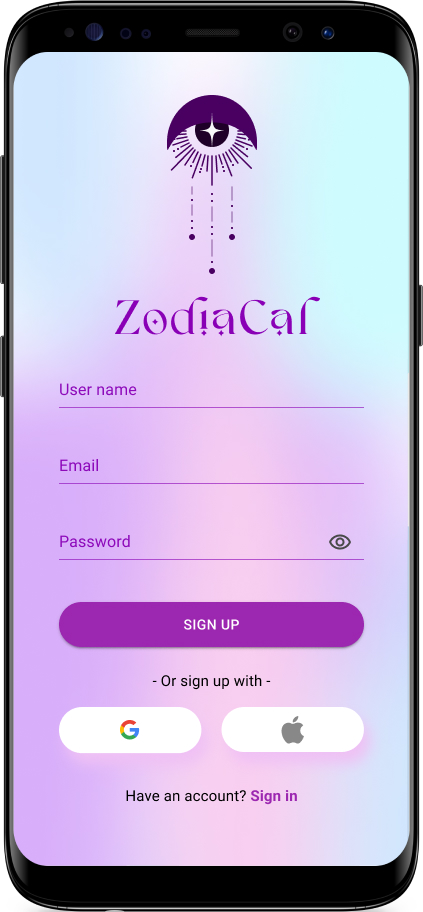
\includegraphics[height=10cm,           keepaspectratio]{images/interfejs_figma/Sign_up}
		\caption{Ekran rejestracji}
		\label{fig:Sign-up}
	\end{minipage}
\end{figure}

\section{Projekt ekranu logowania}
Ekran logowania (Rys. \ref{fig:Sign-in}) przedstawia minimalistyczny formularz logowania do aplikacji, który zawiera dwa pola umożliwiające wprowadzeniu tekstu typu TextInput. TextInputy są interaktywne, to znaczy, że reagują na dane wpisane przez użytkownika. Takie rozwiązanie pozwala na komunikację klienta z aplikacją w celu uniknięcia błędów podczas wpisywania tekstu oraz frustracji użytkownika, który bez komunikatu nie wiedziałby co się dzieje na ekranie. Pole z hasłem ma ikonę oczka, dzięki której można podejrzeć wpisane hasło. Dodatkowo użytkownik ma możliwość zalogowania się do aplikacji poprzez serwisy społecznościowe takie jak konto Google, czy konto Apple. Jeśli klient nie ma jeszcze zarejestrowanego konta może przejść do ekranu rejestracji klikając w przycisk „Sign up”.

\section{Projekt ekranu rejestracji}
Rejestracja użytkownika (Rys. \ref{fig:Sign-up}) odbywa się poprzez uzupełnienie trzech pól w formularzu. Podobnie jak w przypadku ekranu logowania pole „Password” posiada ikonę oczka oraz możliwe jest utworzenie konta z wykorzystaniem innych kont społecznościowych. Po poprawnym wprowadzeniu danych i kliknięciu przycisku „Sign up”, użytkownik zostaje
przeniesiony do ekranu głównego aplikacji.

\begin{figure}[t]
	\begin{center}
		\begin{minipage}{0.4\textwidth}
			\centering
			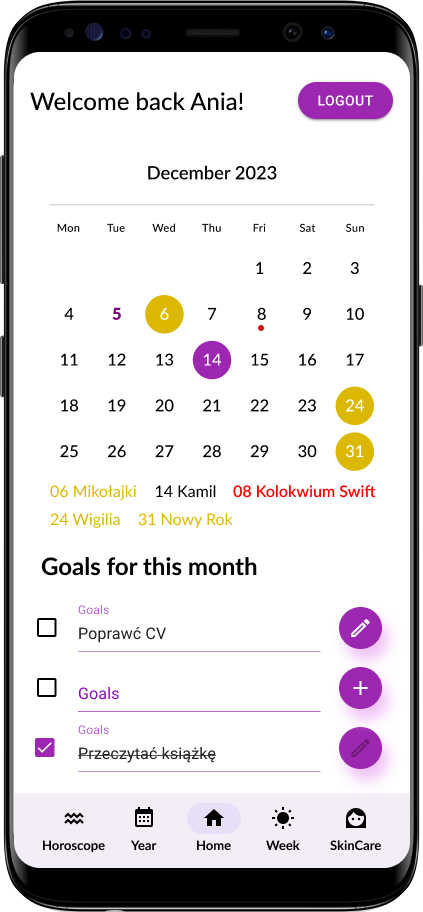
\includegraphics[height=10cm, keepaspectratio]{images/interfejs_figma/Home}
			\caption{Ekran główny}
			\label{fig:Home}
		\end{minipage}
	\end{center}
\end{figure}

\section{Projekt ekranu głównego}
Po udanym zalogowaniu się do aplikacji, użytkownik jest powitany spersonalizowanym komunikatem, który zawiera jego imię (Rys. \ref{fig:Home}). Dodatkowo w tej samej płaszczyźnie znajduję się przycisk do wylogowania. Poniżej znajduję się kalendarz miesięczny z zaznaczonymi świętami, wydarzeniami oraz urodzinami użytkownika. Wygubiony numer w kolorze fioletowym reprezentuje obecny dzień, numer w żółtym kole oznacza święto, numer w fioletowym kole informuje o urodzinach bliskich, mała czerwona kropeczka pod numerem wskazuje na nadchodzące wydarzenie. Pod kalendarzem zostały umieszczone wszystkie informację o zaznaczonych polach w kalendarzu. Dodatkowo poniżej znajduje się sekcja „Goals for this month” w której użytkownik może wprowadzić trzy cele, które chciałby osiągnąć w danym miesiącu. Każde pole posiada checkbox, który informuje, czy klient ukończył cel, jeśli tak checkbox zostaje wypełniony kolorem fioletowym, a tekst w polu zostaje przekreślony, opcja edytowania tekstu zostaje wyłączona. Po prawej stronie znajdują się okrągłe przyciski. Jeśli pole jest puste, przyciski reprezentuje plusik, jeśli w polu już cos się znajduje ikona zmienia się na ołówek, co oznacza, że pole można edytować. W całej aplikacji została wprowadzona nawigacja dolna. Zawiera ona ikony i nazwy odzwierciedlające dostępne ekrany. Zawsze aktualny ekran jest wyróżniony w pasku nawigacyjnym.

\begin{figure}[t]
	\begin{minipage}{0.4\textwidth}
		\centering
		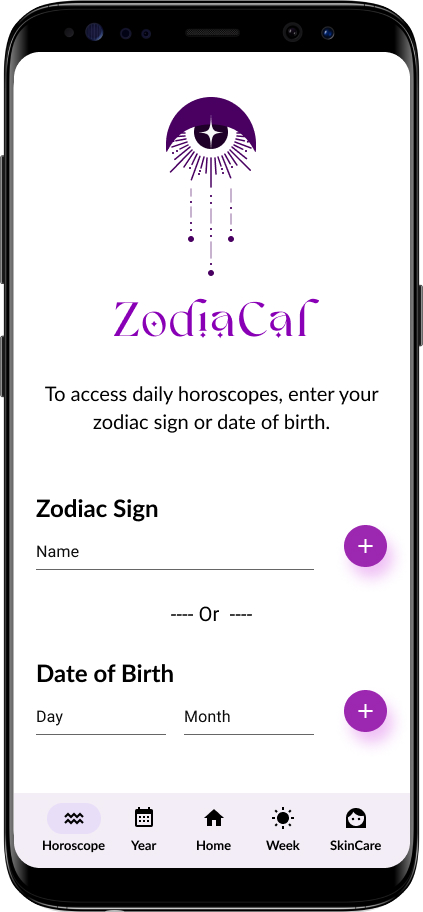
\includegraphics[height=10cm, keepaspectratio]{images/interfejs_figma/Horoscope-onboarding}
		\caption{Onboarding horoskopu}
		\label{fig:Onboarding}
	\end{minipage}
	\hfill
	\begin{minipage}{0.4\textwidth}
		\centering
		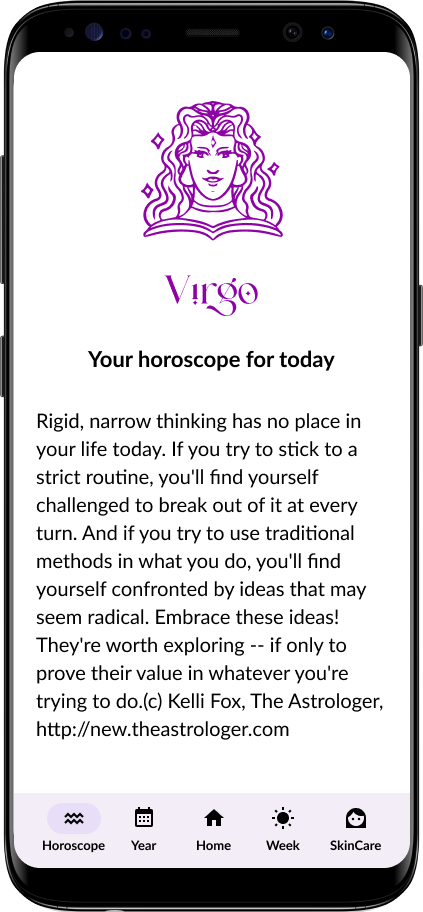
\includegraphics[height=10cm,           keepaspectratio]{images/interfejs_figma/Horoscope}
		\caption{Ekran dziennego horoskopu}
		\label{fig:Horoscope}
	\end{minipage}
\end{figure}

\section{Projekt ekranu horoskopu}
Pierwszą zakładką w nawigacji jest ekran horoskopu, który może wyglądać na dwa sposoby w zależności od tego, czy użytkownik wprowadził swój znak zodiaku do systemu.

Pierwszy scenariusz został ukazany na rysunku \ref{fig:Onboarding}. Jeśli klient uruchamia tę zakładkę po raz pierwszy, jego oczom ukaże się logo aplikacji oraz dwa małe formularze. Użytkownik, jeśli zna swój znak zodiaku może go wprowadzić w pierwszym formularzu. Jeśli jednak dopiero rozpoczyna swoją przygodę z horoskopami, aplikacja pomoże mu określić swój znak zodiaku. Wystarczy podać dzień i miesiąc urodzenia, a program sam przydzieli znak zodiaku i wyświetli go na ekranie wraz z horoskopem.

Rysunek \ref{fig:Horoscope} przedstawia sytuację, gdzie w systemie już znajduję się informacja o znaku zodiaku użytkownika. Logo aplikacji zostaje zamienione na ilustrację przetrawiającą wersję graficzną znaku zodiaku. Ilustracje wszystkich znaków zostały pobrane ze strony Freepik.com, który posiada darmową licencję do korzystania z zasobów znajdujących się na stronie w zakresie niekomercyjnym. Każdego dnia na tym ekranie pojawia się inna wróżba zodiaku.

\begin{figure}[t]
	\begin{minipage}{0.4\textwidth}
		\centering
		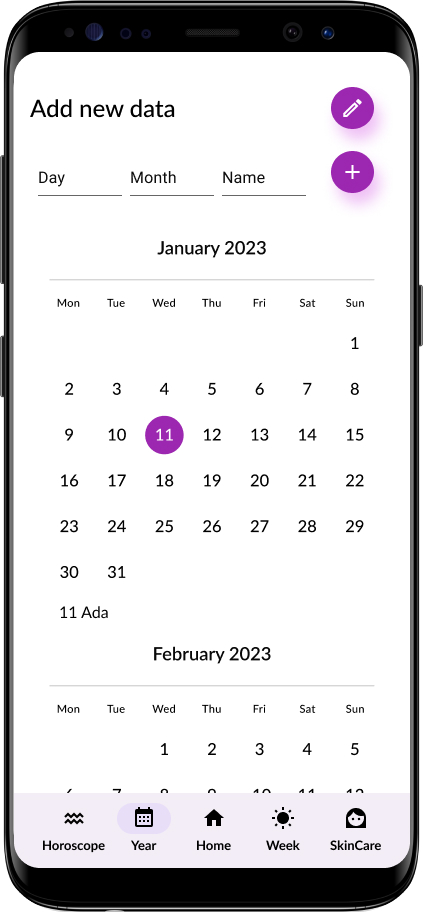
\includegraphics[height=10cm, keepaspectratio]{images/interfejs_figma/Year}
		\caption{Widok kalendarza rocznego}
		\label{fig:Year}
	\end{minipage}
	\hfill
	\begin{minipage}{0.4\textwidth}
		\centering
		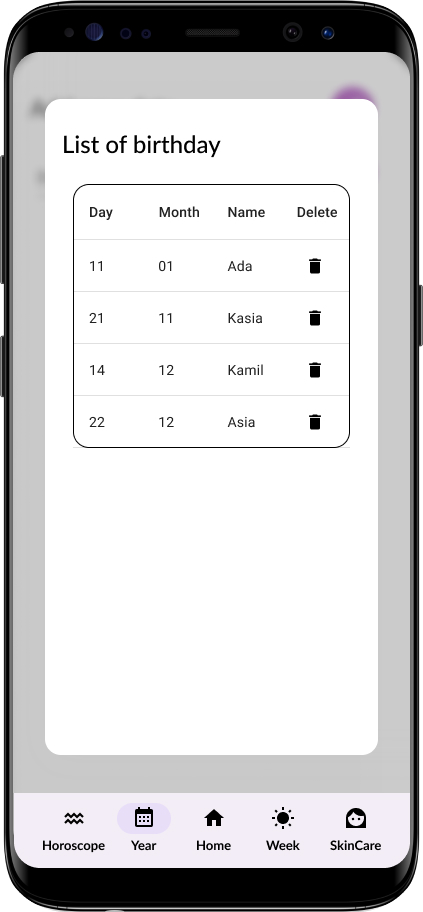
\includegraphics[height=10cm,           keepaspectratio]{images/interfejs_figma/Birthday-Edit}
		\caption{Ekran listy dat urodzin}
		\label{fig:Birthday}
	\end{minipage}
\end{figure}

\section{Projekt widoku kalendarza rocznego}
Kolejna zakładka o nazwie „Year” przenosi użytkownika do widoku kalendarza rocznego \ref{fig:Year}). W tym ekranie wyświetlane są kalendarze miesięcy jedynie danego roku. Dzięki takiemu rozwiązaniu klient nie musi się przejmować zbędnym skorolowaniem, które może omyłkowo zaprowadzić go do zupełnie innego roku. W tym widoku kalendarza zaznaczone są jedynie święta oraz urodziny. Poniżej każdego kalendarza na dany miesiąc znajduję się informacja o zaznaczonych polach. Na górze ekranu został umieszczony formularz do dodawania urodziny do listy użytkownika. Zawiera on trzy pola: day, month oraz name. Po prawej stronie znajduje się przycisk dodawania urodzin do listy. Jeśli użytkownik się pomyli lub
po prosu będzie chciał edytować listę z datami, musi kliknąć w okrągły przycisk z ikoną ołówka. Otworzy się wtedy tak zwany portal (Rys. \ref{fig:Birthday}) przedstawiający tabelę z czterema kolumnami: day, month, name i delete. To właśnie tam użytkownik może usunąć złe rekordy. Tabela sortuję się w taki sposób, aby na początku zawsze były pola z poprawną kolejnością miesięcy, a następnie w sposób rosnący reprezentuje kolejność dni w miesiącu.

\begin{figure}[t]
	\begin{minipage}{0.4\textwidth}
		\centering
		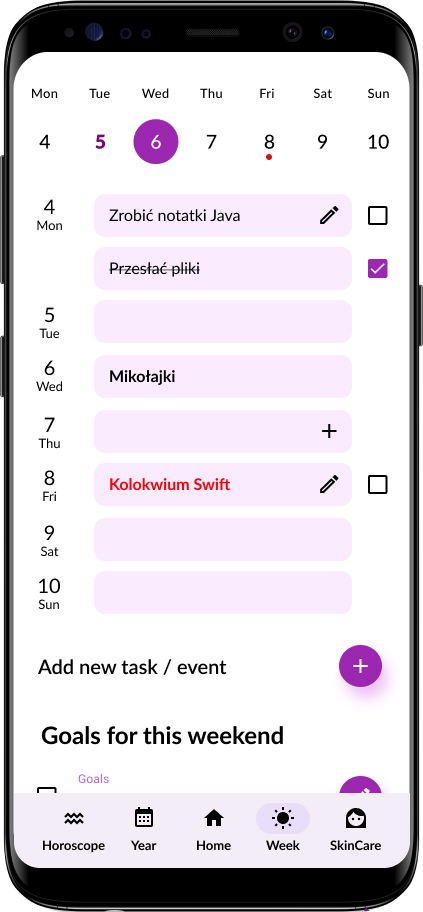
\includegraphics[height=10cm, keepaspectratio]{images/interfejs_figma/Week}
		\caption{Widok kalendarza tygodniowego}
		\label{fig:Week}
	\end{minipage}
	\hfill
	\begin{minipage}{0.4\textwidth}
		\centering
		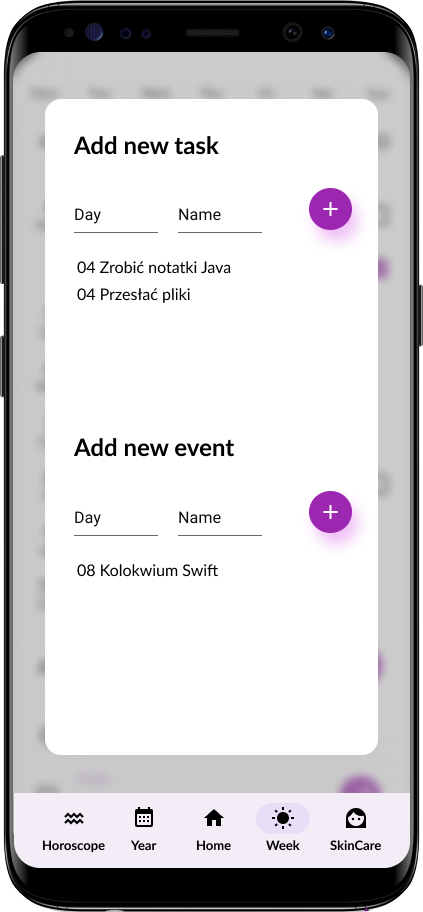
\includegraphics[height=10cm,           keepaspectratio]{images/interfejs_figma/Task_Event}
		\caption{Ekran dodawania zadań i wydarzeń do kalendarza}
		\label{fig:Task_Event}
	\end{minipage}
\end{figure}

\section{Projekt widoku kalendarza tygodniowego}
Rysunek \ref{fig:Week} reprezentuje ekran zakładki „Week”. W tym widoku  użytkownik może podglądać swoje zadania i wydarzenia na konkretny tydzień. Na samej górze znajduje się kalendarz z pogrubionym obecnym dniem, zaznaczonym świętem i wydarzeniem. Poniżej dla każdego dnia zostają wyświetlone zdania i wydarzenia, które użytkownik wprowadził na dany dzień. Klient może edytować pola zadań i wydarzeń poprzez kliknięcie ikony ołówka. Inputy mają takie samo zachowanie jak w przypadku komponentu Goals w ekranie głównym. Na samym dole znajduje się miejsce na wpisanie przez użytkownika celów na ten tydzień.

Aby dodać zadanie lub wydarzenie należy kliknąć okrągły przycisk z plusem. Po tej akcji pojawi się portal z formularzem do tworzenia zadań i wydarzeń (Rys. \ref{fig:Task_Event}). Jest to bardzo minimalistyczny interfejs zawierający dwa TextInput day i name oraz przycisk dodawania. Aby zachować spójność projektu poniżej każdego z formularzy znajduje się tabela z trzema kolumnami: day, name, delete. Z tego miejsca użytkowni może zarządzać swoimi zadaniami oraz wydarzeniami na dany tydzień. Tabela sortuje rekordy w sposób rosnący.

\begin{figure}[t]
	\begin{center}
		\begin{minipage}{0.4\textwidth}
			\centering
			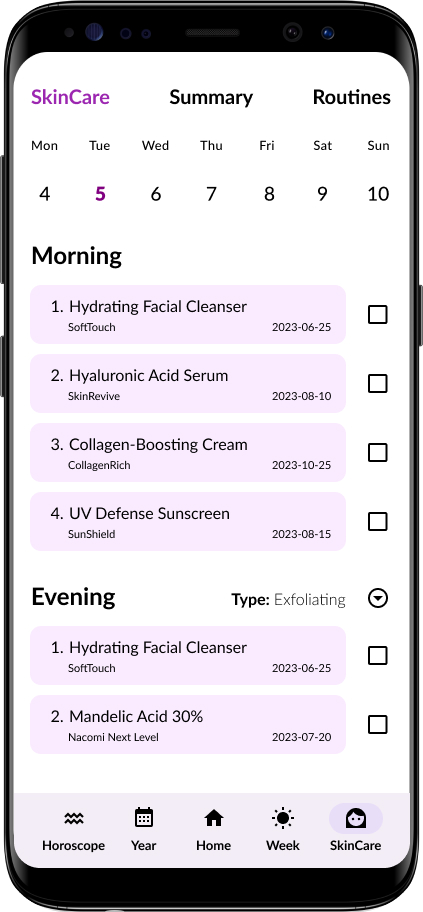
\includegraphics[height=10cm, keepaspectratio]{images/interfejs_figma/SkinCare}
			\caption{Ekran pielęgnacji na dany dzień}
			\label{fig:SkinCare}
		\end{minipage}
	\end{center}
\end{figure}

\section{Projekt ekranu pielęgnacji}
Ostatnią zakładką w pasku nawigacyjnym jest SkinCare (Rys. \ref{fig:SkinCare}). Podobnie jak w ekranie widoku kalendarza tygodniowego na górze znajduje się kalendarz tygodniowy, z tym że na nim nie ma już zaznaczonych żadnych świąt, wydarzeń czy zadań. Dodatkowo klikając w poszczególne dni na kalendarzu poniżej wyświetla się pielęgnacja dedykowana na konkretny dzień, w ekranie widoku kalendarza tygodniowego, wszystkie zadania, wydarzenia, święta są wyświetlane razem. Pielęgnacja jest podzielona na dwie sekcje: pielęgnację poranną i pielęgnację wieczorną. Pielęgnacja na dzień zawsze zawiera te same produkty, chyba że użytkownik sam je zmieni, natomiast pielęgnacja na wieczór jest wybierana z wysuwanego menu z którego można wybrać jedną z czterech typów pielęgnacji: nawilżająca, złuszczająca, regeneracyjna lub przerwa. W zależności od tego jaką pielęgnacje użytkownik wybierze taka lista produktów zostanie wyświetlona w sekcji pielęgnacji wieczornej. Dodatkową funkcją jest możliwość kliknięcia przez użytkownika checkboxa, gdy wykorzystał produkt z wymienionej listy. Na samej górze znajduję się osobna mini nawigacja dla sekcji SkinCare. Aktualny widok jest zaznaczony kolorem fioletowym w nawigacji.

\begin{figure}[t]
	\begin{minipage}{0.4\textwidth}
		\centering
		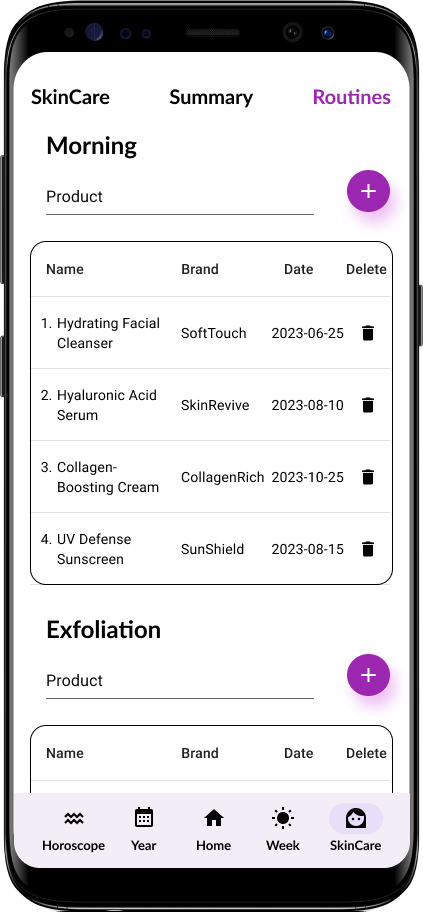
\includegraphics[height=10cm, keepaspectratio]{images/interfejs_figma/SkinCare-Routines}
		\caption{Ekran tworzenia rutyny pielęgnacyjnej}
		\label{fig:Routines}
	\end{minipage}
	\hfill
	\begin{minipage}{0.4\textwidth}
		\centering
		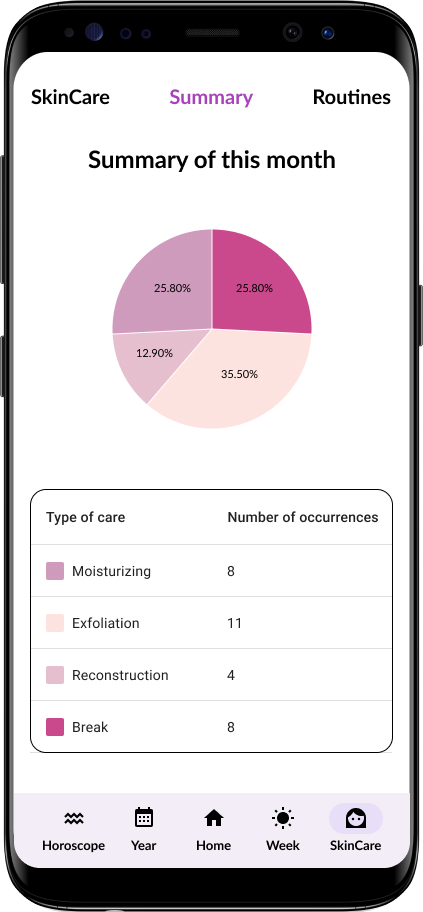
\includegraphics[height=10cm,           keepaspectratio]{images/interfejs_figma/SkinCare-Summary}
		\caption{Ekran podsumowania miesiąca pielęgnacji}
		\label{fig:Summary}
	\end{minipage}
\end{figure}

Początkowo sekcja pielęgnacji porannej i wieczornej jest pusta, aby dodać kosmetyki należy kliknąć Rutines w górnej nawigacji. Po wykonaniu tego kroku użytkownikowi ukażą się formularze z nagłówkiem oraz polem do wpisania (Rys. \ref{fig:Routines}). Podczas wpisywania nazwy klient będzie mógł wybrać z bazy danych konkretne produkty. Po dodaniu produktu poniżej zostanie zaktualizowana tabela z listą produktów do danej pielęgnacji. W tabeli znajdują się cztery kolumny: name, brand, date oraz delete. Dla każdej sekcji jest osobny formularz oraz tabela. Ostatnim ekranem jest widok podsumowania pielęgnacji na dany miesiąc (Rys. \ref{fig:Summary}).

W tym miejscu są wyświetlane informacja w jakim stopniu pielęgnacja w tym miesiącu była nawilżająca, złuszczająca, regeneracyjna lub wystąpiła przerwa. Na środku znajduję się graf kołowy z wypisanymi procentami, a poniżej tabela z dwiema kolumnami: „Type of care” stanowiąca również legendę do wykresu oraz  „Number of occurrences”, która wyświetla ile razy dana pielęgnacja wystąpiła w miesiącu.

